	\chapter{Kravspecifikation}
	
			\section{Systembeskrivelse}
		Systemet består af en database med brugeradgang via iOS applikation.
		Databasen indeholder brugere, projekter, PDF tegninger og data om projekterne.
		Et projekt indeholder en PDF tegning, tegne objekter, mulighed for upload af billede og tekst.
		
		\begin{figure}[H]
			\centering
			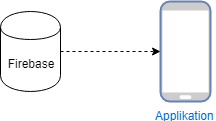
\includegraphics[width=0.4\linewidth]{Kravspecifikation/Oversigtoversystem}
			\caption{Oversigt over systemet}
			\label{fig:OversigtSystembeskrivelse}
		\end{figure}
		
		Systemet skal kunne håndtere de bygge projekter Rambøll har, og oprette nye når de overtager et nyt bygge projekt.
		Disse skal kunne tilgåes af Rambøll ansatte, via enten en smartphone eller tablet.
		Rambøll ansatte får tildelt et personligt login.
		Brugere skal kunne oprette en registring for et givet projekt.
		Når en bruger er færdig med at oprette sin registrering, skal denne kunne exportes til en excel fil og sendes som en vedhæftet fil i en mail.
		Systemet har en log, som indeholder en liste over alle registreringer, til et givent projekt. \\	
				
		\clearpage

	
	\section{User stories} 
	Følgende er en kort beskrivelse af must user stories til Rambølls Tilsyns App, som er fundet sammen med Rambøll ved hjælp af MoSCoW analyse. \cite{MoSCoW} For alle user stories fuldt beskrevet med Gherkin, se kravspecifikationen afsnit \vref{Krav-sec:UserStories}.
	Aktør kontekst diagram findes i kravspecifikationen afsnit \vref{Krav-sec:Aktor}.

	\subsection*{Log-in (CRS-1)}
	Som bruger\\
	Ønsker jeg at kunne logge ind på applikationen\\
	For at kunne benytte applikationen
	
	\subsection*{Opret bruger (CRS-2)}
	Som ejer\\
	Ønsker jeg at kunne oprette bruger på applikationen\\
	For at kunne give montører samt kunder adgang til systemet
	
	\subsection*{Opret en registrering på PDF tegning (CRS-4)}
	Som bruger\\
	Ønsker jeg at kunne ændre brugeroplysninger\\
	For at have aktuelle oplysninger på applikationen
	
	\subsection*{Opret fluebens opbjekt på PDF tegning (CRS-5)}
	Som ejer eller montør\\
	Ønsker jeg at kunne oprette en sag\\
	For kunne lave en fejlmelding på et given lyskryds

	\subsection*{Opret billede opbjekt på PDF tegning (CRS-6)}
	Som montør\\
	Ønsker jeg at kunne tage en sag\\
	For at kunne lave en reparation på et fejlmeldt lyskryds
	
	\subsection*{Opret tekstfelt opbjekt på PDF tegning (CRS-7)}
	Som montør\\
	Ønsker jeg at kunne ændre en sags driftstatus\\
	For at kunne holde Strøm Hansen og Randers kommune opdateret på reparatoioner af lyskryds
	
	\subsection*{Opret minus opbjekt på PDF tegning (CRS-11)}
	Som bruger\\
	Ønsker jeg at kunne skrive kommentar til en given sag\\
	For at kunne skrive kommentar på eventuelle mangler, feedback og til korrespondance mellem de forskellige brugere.

	\subsection*{Slet opbjekt på PDF tegning (CRS-12)}
	Som bruger\\
	Ønsker jeg at kunne sortere sager\\
	For at give et hurtigt overblik hvis en specifik sag ønskes fundet

	\subsection*{Afslut registrering på PDF tegning (CRS-13)}
	Som bruger\\
	Ønsker jeg at kunne danne mig et hurtigt overblik ved hjælp af en map funktion\\
	For at kunne se et overbliks billede af alle lyskryds i Randers kommune  og deres nuværende status
	
	\subsection*{Opret projekt (CRS-16)}
	Som kunde og ejer\\
	Ønsker jeg at modtage notifikationer når en driftstatus ændre sig på et lyskryds ændre sig\\
	For at få opdateringer hvis et lyskryds ændre driftstatus \\
	

	\section{Ikke funktionelle krav}
	\begin{itemize}[-]
		\itemsep 0.3em 
		\item Skal kunne tilgås gennem en Web applikation og Android applikation
		\item Der skal anvendes Microsoft teknologier og software
		\item Alle brugere skal kunne anvende systemet på samme tid. Maks antal enheder er 10 på samme tid %\\
		%\item Systemet skal have svartider under 500ms ved 99\% af requests på en dansk kablet internetforbindelse
		%\item Systemet skal have en oppetid på 99,7\%, målt over 3 måneder
		%\item Database og web-server skal være køre på hver deres server
	\end{itemize}


\section{Afgrænsning}
Projektet har en naturlig begrænsning i form af den korte tid fra idé til produkt, som er gældende for bachelorprojekter.\\
Smartphone applikationen vil blive udviklet ved anvendelse af Xamarin, det muliggør at skrive i C\# og er et cross platform SDK som gør det muligt at udvikle til både iOS og Android. \\
Applikationen som bliver udviklet til iOS i første omgang, da dette er Rambølls ønske. \\
Derudover er der til projektet lavet en Firebase database, for at mindske database problemer til udviklingen af appliaktionen og ikke påvirke Rambølls nuværende database.

\subsection{User stories, prioriteret efter MoSCoW}
Der er i samarbejde med Rambøll også lavet en MoSCoW \cite{MoSCoW} analyse, for at prioriter funktionaliteten, som følgende: \\
\textbf{Must:} Opret en registrering på PDF tegning (CRS-4) \\
\textbf{Should:} Opret cirkel opbjekt på PDF tegning (CRS-10) \\
\textbf{Could:} Opret en registrering uden PDF tegning (CRS-14) \\
Must er funktionalitet af højeste prioritet, derefter er det Should og tilsidst er det Could. \\
For den fulde MoSCoW analyse se \vref{Dok-sec:MoSCoW} i dokumentationen. 
	